\chapter{Advanced use of graphs}
\label{chap-advanced-grammars}
\section{Types of graphs}
\index{Graph!types of}\index{Types of graphs}
Unitex can handle several types of graphs that correspond to the following
uses: automatic inflection of dictionaries, preprocessing of texts, normalization
of text automata, dictionary graphs, search for patterns, disambiguation and
automatic graph generation. These different types of graphs are not interpreted
in the same way by Unitex. Certain operations, like transduction, are allowed for
some types and forbidden for others. In addition, special symbols are not the
same depending on the type of graph. This section presents each type of graph
and shows their peculiarities.

\subsection{Inflection transducers}
\index{Transducer!inflection}\index{Automatic inflection}
An inflection transducer describes the morphological variation that is associated
with a word class by assigning inflectional codes to each variant. The paths of
such a transducer describe the modifications that have to be applied to the canonical
forms and the corresponding outputs contain the inflectional information that will be
produced.

\bigskip
\begin{figure}[!h]
\begin{center}
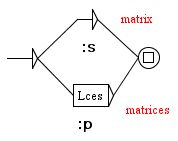
\includegraphics[width=4.5cm]{resources/img/fig6-1.png}
\caption{Example of an inflectional grammar}
\end{center}
\end{figure}

\index{Operator!\verb+L+}
\index{Operator!\verb+R+}
\index{Operator!\verb+C+}
\index{Operator!\verb+D+}
\index{Operator!\verb+U+}
\index{Operator!\verb+P+}
\index{Operator!\verb+W+}
\index{\verb+L+}
\index{\verb+R+}
\index{\verb+C+}
\index{\verb+D+}
\index{\verb+U+}
\index{\verb+P+}
\index{\verb+W+}
\noindent The paths may contain operators and letters. The possible operators
are represented by the characters \verb+L+, \verb+R+, \verb+C+, \verb+D+, 
\verb+U+,\verb+P+ and \verb+W+.
All letters that are not operators are characters. The only
allowed special symbol is the empty word \verb+<E>+.\index{\verb+<E>+} It is not
possible to refer to information in dictionaries in an inflection transducer,
but it is possible to reference subgraphs.

\bigskip
\noindent Transducer outputs are concatenated in order to produce a string of
characters. This string is then appended to the produced dictionary entry.
Outputs with variables do not make sense in an inflection transducer.

\bigskip
\noindent Case of letters is respected: lowercase letters stay lowercase, 
the same for uppercase letters. Besides,
the connection of two boxes is exactly equivalent to the concatenation of their
contents together with the concatenation of their outputs.
(cf.
figure~\ref{fig-equivalent-inflection-paths}).\index{Respect!of
lowercase/uppercase}

\bigskip
\begin{figure}[!h]
\begin{center}
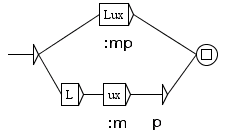
\includegraphics[width=5.5cm]{resources/img/fig6-2.png}
\caption{Two equivalent paths in an inflection grammar\label{fig-equivalent-inflection-paths}}
\end{center}
\end{figure}

\bigskip
\noindent Inflection transducers may be compiled before being used by the
inflection program. If not, the inflection program will compile them on the fly.

\bigskip
\noindent For more details, see section
\ref{section-automatic-inflection}.

\subsection{Preprocessing graphs}
\index{Text!preprocessing}\index{Grammars!for phrase boundary recognitions}
\index{Grammars!normalisation!of non-ambiguous forms}
Preprocessing graphs are meant to be applied to texts before they are
tokenized into lexical units. These graphs can be used for inserting or
replacing sequences in the texts. The two customary uses of these graphs are
normalization of non-ambiguous forms and sentence boundary recognition.

\bigskip
\noindent The interpretation of these graphs in Unitex is very close to that of
syntactic graphs used by the search for patterns. The differences are the following:
\begin{itemize}
  \item you can use the special symbol \verb+<^>+ that recognizes a newline;\index{\verb+<^>+}
  \item if you work in character by character mode, you can use the special
  symbol \verb+<L>+ that recognizes one letter, as defined in
  the alphabet file;\index{\verb+<L>+}
  \item it is impossible to refer to information in dictionaries;
  \item it is impossible to use morphological filters;
  \item it is impossible to use morphological mode;
  \item it is impossible to use contexts.
\end{itemize}

The figures~\ref{fig-example-sentence-splitting} (page
\pageref{fig-example-sentence-splitting})
and~\ref{fig-normalization-grammar} (page
\pageref{fig-normalization-grammar}) show examples of preprocessing graphs.


\subsection{Graphs for normalizing the text automaton}
\label{section-normalizing-text-automataon}
\index{Automaton!text}\index{Text!normalisation of the automaton}
\index{Grammars!normalisation!of the text automaton}
\index{Normalization!of the text automaton}
\index{Normalization!of ambiguous forms}
Graphs for normalizing the text automaton allow you to normalize
ambiguous forms. They can describe several labels for the same form.
These labels are then inserted into the text automaton thus making the
ambiguity explicit. Figure~\ref{fig-tfst-normalization-grammar} shows an
extract of the normalization graph used by default for French.

\bigskip
\begin{figure}[!h]
\begin{center}
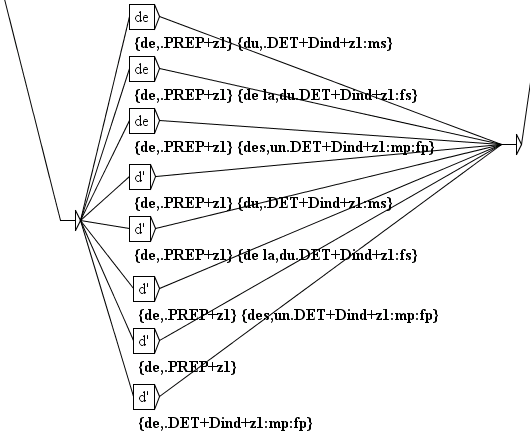
\includegraphics[width=13.5cm]{resources/img/fig6-3.png}
\caption{Extract of the normalization graph used for French\label{fig-tfst-normalization-grammar}}
\end{center}
\end{figure}

\noindent The paths describe the forms that have to be normalized. Lower case
and upper case variants are taken into account according to the following principle:
uppercase letters in the graph only recognize uppercase letters in the
text automaton;  lowercase letters can recognize both lowercase and uppercase
letters. \index{Case respect}

\bigskip
\noindent The transducer outputs represent the sequences of labels that will be
inserted into the text automaton. These labels can be dictionary entries or strings 
of characters. The labels that
represent dictionary entries have to respect the DELAF format 
and must be enclosed by the \verb+{+ and \verb+}+ symbols. Outputs
with variables do not make sense in this kind of graph.
You cannot use morphological filters, morphological mode or contexts.

\bigskip
\noindent It is possible to reference subgraphs. It is not possible to reference
information in dictionaries in order to describe the forms to normalize. The only special
symbol that is recognized in this type of graph is the empty word
\verb+<E>+.\index{\verb+<E>+} The graphs for normalizing ambiguous forms need to
be compiled before using them.


\subsection{Syntactic graphs}
\index{Graph!syntactic}\index{Grammars!local}
Syntactic graphs, often called local grammars, allow you to describe syntactic
patterns that can then be searched in the texts. Of all kinds of graphs these
have the greatest expressive power because they allow you to refer to information
in dictionaries. \index{Reference to information in the
dictionaries}\index{Dictionaries!reference to information in the}

\bigskip
\noindent Lower case/upper case variants may be used according to the principle described
above. It is still possible to enforce respect of case by enclosing an
expression in double quotes. The use of double quotes also allows you to enforce
the respect of spaces. In fact, Unitex by default assumes that a space is possible between two
boxes. In order to enforce the presence of a space you have to enclose it in
double quotes. For prohibiting the presence of a space you have to use the
special symbol \verb+#+.\index{\verb+#+}
\index{Respect!of lowercase/uppercase}\index{Case!see {Respect!of
lowercase/uppercase}}
\index{Lowercase!see {Respect!of lowercase/uppercase}}
\index{Uppercase!see {Respect!of lowercase/uppercase}}
\index{Respect!of spaces}

\bigskip
\noindent Syntactic graphs can reference subgraphs (cf.
section~\ref{section-subgraphs}). They also have outputs including outputs
with variables. The produced sequences are interpreted as strings of characters
that will be inserted in the concordances or in the text if you want to modify it
(cf. section~\ref{section-modifying-text}).

\bigskip
\noindent Syntactic graphs can use contexts (see section
\ref{section-contexts}).

\bigskip
\noindent Syntactic graphs can use morphological filters (see section
\ref{section-filters}).

\bigskip
\noindent Syntactic graphs can use morphological mode (see section
\ref{section-morphological-mode}).

\bigskip
\noindent The special symbols that are supported by the syntactic graphs are the same as those that
are usable in regular expressions (cf.
section~\ref{section-special-symbols}).

\bigskip
\noindent It is not obligatory to compile syntactic graphs before using them for
pattern matching. If a graph is not compiled the system will compile it
automatically.

\subsection{ELAG grammars}
\index{Grammars!ELAG}\index{ELAG}

ELAG grammars for disambiguation between lexical symbols in text automata are
described in section \ref{section-elag-grammars}, page
\pageref{section-elag-grammars}.


\subsection{Parameterized graphs}
\index{Graph!parameterized}
Parameterized graphs are meta-graphs that allow you to generate a family of graphs
using a lexicon-grammar table. It is possible to construct parameterized
graphs for all possible kinds of graphs. The construction and use of parameterized
graphs are explained in chapter~\ref{chap-lexicon-grammar}.

\section{Compilation of a grammar}
\label{section-graph-compilation}
\subsection{Compilation of a graph}
\index{Graph!compilation}\index{Compilation of a graph}
Compilation is the operation that converts the \verb+.grf+ format
to a format that can be manipulated more easily  by Unitex programs. In order to
compile a graph, you must open it and then click on "Compile FST2" in the
"Tools" submenu of the menu "FSGraph". Unitex then launches the 
\verb+Grf2Fst2+ program.\index{\verb+Grf2Fst2+}\index{External
programs!\verb+Grf2Fst2+} You can keep track of its execution in a 
window (cf. Figure~\ref{fig-compilation-frame}).

\bigskip
\begin{figure}[!h]
\begin{center}
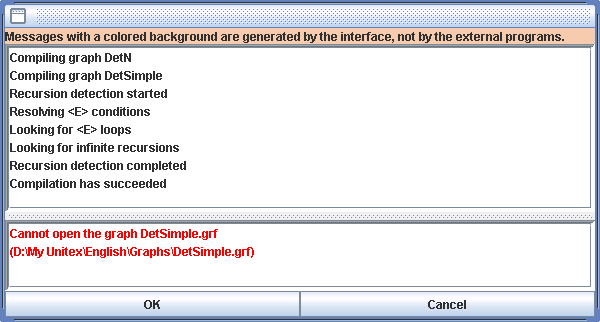
\includegraphics[width=14.7cm]{resources/img/fig6-4.png}
\caption{Compilation window\label{fig-compilation-frame}}
\end{center}
\end{figure}

\noindent If the graph references subgraphs, those are automatically compiled.
The result is a \verb+.fst2+ file\index{File!\verb+.fst2+} that contains all the graphs
that make up a grammar. The grammar is then ready to be used by Unitex programs.

\subsection{Approximation with a finite state transducer}
\index{Graph!approximation with a finite state transducer}
\index{Approximation of a grammar with a finite state transducer}
\index{\verb+Flatten+}\index{External programs!\verb+Flatten+}
The FST2 format conserves the architecture in subgraphs of the grammars, which
is what makes them different from strict finite state transducers. The 
\verb+Flatten+ program allows you to turn a FST2 grammar into a finite
state transducer whenever this is possible, and to construct an approximation if not.
This function thus permits to obtain objects that are easier to manipulate and
to which all classical algorithms on automata can be applied.

\bigskip
\noindent In order to compile and thus transform a grammar, select the command
"Compile \& Flatten FST2" in the "Tools" submenu of the "FSGraph" menu. The
window of Figure~\ref{fig-flatten-configuration} allows you to
configure the approximation process.

\bigskip
\begin{figure}[!h]
\begin{center}
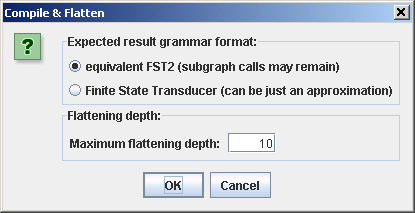
\includegraphics[width=10.4cm]{resources/img/fig6-5.png}
\caption{Configuration of approximation of a
grammar\label{fig-flatten-configuration}}
\end{center}
\end{figure}

\noindent The box "Flattening depth" lets you specify the level of embedding of
subgraphs. This value represents the maximum depth up to which the callings of
subgraphs will be replaced by the subgraphs themselves.

\bigskip
\noindent The "Expected result grammar format" box allows you to determine the
behavior of the program beyond the selected limit. If you select the "Finite State
Transducer" option, the calls to subgraphs will be replaced by \verb+<E>+
beyond the maximum depth. This option guarantees that we obtain a finite state transducer,
however possibly not equivalent to the original grammar. On the contrary, the
"equivalent FST2" option indicates that the program should allow for subgraph
calls beyond the limited depth. This option guarantees the strict equivalence of
the result with the original grammar but does not necessarily produce a finite
state transducer. This option can be used for optimizing certain grammars.

\bigskip
\noindent A message indicates at the end of the approximation process if the result is a
finite state transducer or an FST2 grammar and in the case of a transducer if it
is equivalent to the original grammar (cf.
Figure~\ref{fig-flatten-result}).

\bigskip
\begin{figure}[!h]
\begin{center}
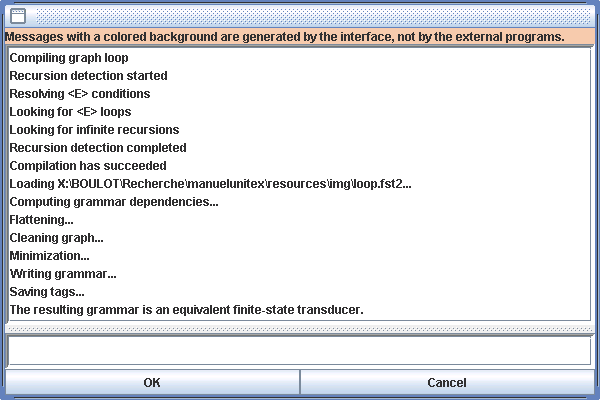
\includegraphics[width=14.7cm]{resources/img/fig6-6.png}
\caption{Resultat of the approximation of a grammar\label{fig-flatten-result}}
\end{center}
\end{figure}




\subsection{Constraints on grammars}
\index{Grammars!constraints}\index{Constraints on grammars}
With the exception of inflection grammars, a grammar can never have an empty
path. This means that the paths of a main graph must not recognize the
empty word but this does not prevent a subgraph of that grammar from recognizing
epsilon.

\bigskip
\noindent It is not possible to associate a transducer output with a call to a
subgraph. Such outputs are ignored by Unitex. It is therefore necessary to use an empty
box that is situated to the left of the call to the subgraph in order to specify the
output (cf. Figure~\ref{fig-subgraph-output}).
\index{Output associated to a subgraph call}

\bigskip
\begin{figure}[!h]
\begin{center}
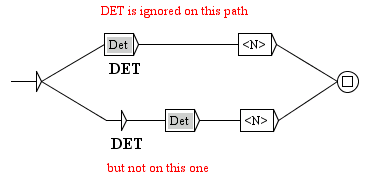
\includegraphics[width=9.1cm]{resources/img/fig6-7.png}
\caption{How to associate an output with a call to a subgraph\label{fig-subgraph-output}}
\end{center}
\end{figure}

\index{Void loops}
\noindent The grammars must not contain void loops because the Unitex programs
cannot terminate the exploration of such a grammar. A void loop is a configuration that
causes the \verb+Locate+ program to enter an infinite loop.
Void loops can originate  from
transitions that are labeled by the empty word or from recursive calls to
subgraphs.

\bigskip
\noindent Void loops due to transitions with the empty word  can have two
origins of which the first is illustrated by the 
Figure~\ref{fig-epsilon-output-loop}.
This type of loops is due to the fact that a transition with the
empty word cannot be eliminated automatically by Unitex because it is associated with an
output. Thus, the transition with the empty word of
Figure~\ref{fig-epsilon-output-loop} will not be suppressed
and will cause a void loop.

\begin{figure}[!h]
\begin{center}
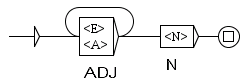
\includegraphics[width=6.2cm]{resources/img/fig6-8.png}
\caption{Void loop due to a transition by the empty word with a
transduction\label{fig-epsilon-output-loop}}
\end{center}
\end{figure}

%\medskip
\noindent The second category of loop by epsilon concerns the call to subgraphs
that can recognize the empty word. This case is illustrated in
Figure~\ref{fig-epsilon-subgraph-loop}: if the subgraph
\verb+Adj+ recognizes epsilon, there is a void loop that Unitex cannot detect.

\begin{figure}[!ht]
\begin{center}
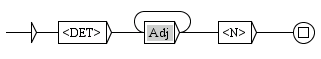
\includegraphics[width=7.9cm]{resources/img/fig6-9.png}
\caption{Void loop due to a call to a subgraph that recognizes epsilon
\label{fig-epsilon-subgraph-loop}}
\end{center}
\end{figure}

%\medskip
\noindent The third possibility of void loops is related to recursive calls to
subgraphs. Look at the graphs \verb+Det+ and \verb+DetCompose+ in
figure~\ref{fig-recursive-calls-loop}.

\begin{figure}[!ht]
\begin{center}
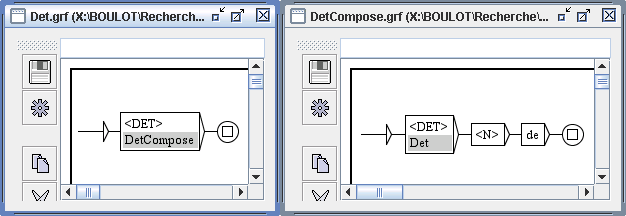
\includegraphics[width=15.5cm]{resources/img/fig6-10.png}
\caption{Void loop caused by two graphs calling each
other\label{fig-recursive-calls-loop}}
\end{center}
\end{figure}

%\medskip
\noindent Each of these graphs can call
the other \textit{without reading any text}. The fact that none of these two
graphs has labels between the initial state and the call to the subgraph is
crucial. In fact, if there were at least one label different from epsilon between
the beginning of the graph \verb+Det+ and the call to \verb+DetCompose+, this
would mean that the Unitex programs exploring the graph \verb+Det+ would have to
read the pattern described by that label in the text before calling
\verb+DetCompose+ recursively. In this case the programs would loop infinitely
only if they  recognized the pattern an infinite number of times in the text,
which is impossible.

\bigskip
\index{Intervals}
\noindent In order to recognize token sequences in which one word or one token of a specific grammatical category appears once, several times or never, you can attach an integer interval to a box.
If you attach the interval [m,M] to a box containing <ADJ>, the path will match sequences with at least $m$ consecutive adjectives and no more than $M$.
Intervals are attached by inserting \verb+$[m,M]$+ into the output of the box, just after the character ``/'', and according to the following rules : 
\begin{itemize}
\item \verb+[m,M]+ = at least $m$ consecutive terms and no more than $M$
\item \verb+[,M]+ = 0 to $M$  
\item \verb+[m,]+ = at least $m$
\end{itemize}

\begin{figure}[h!]
\begin{center}
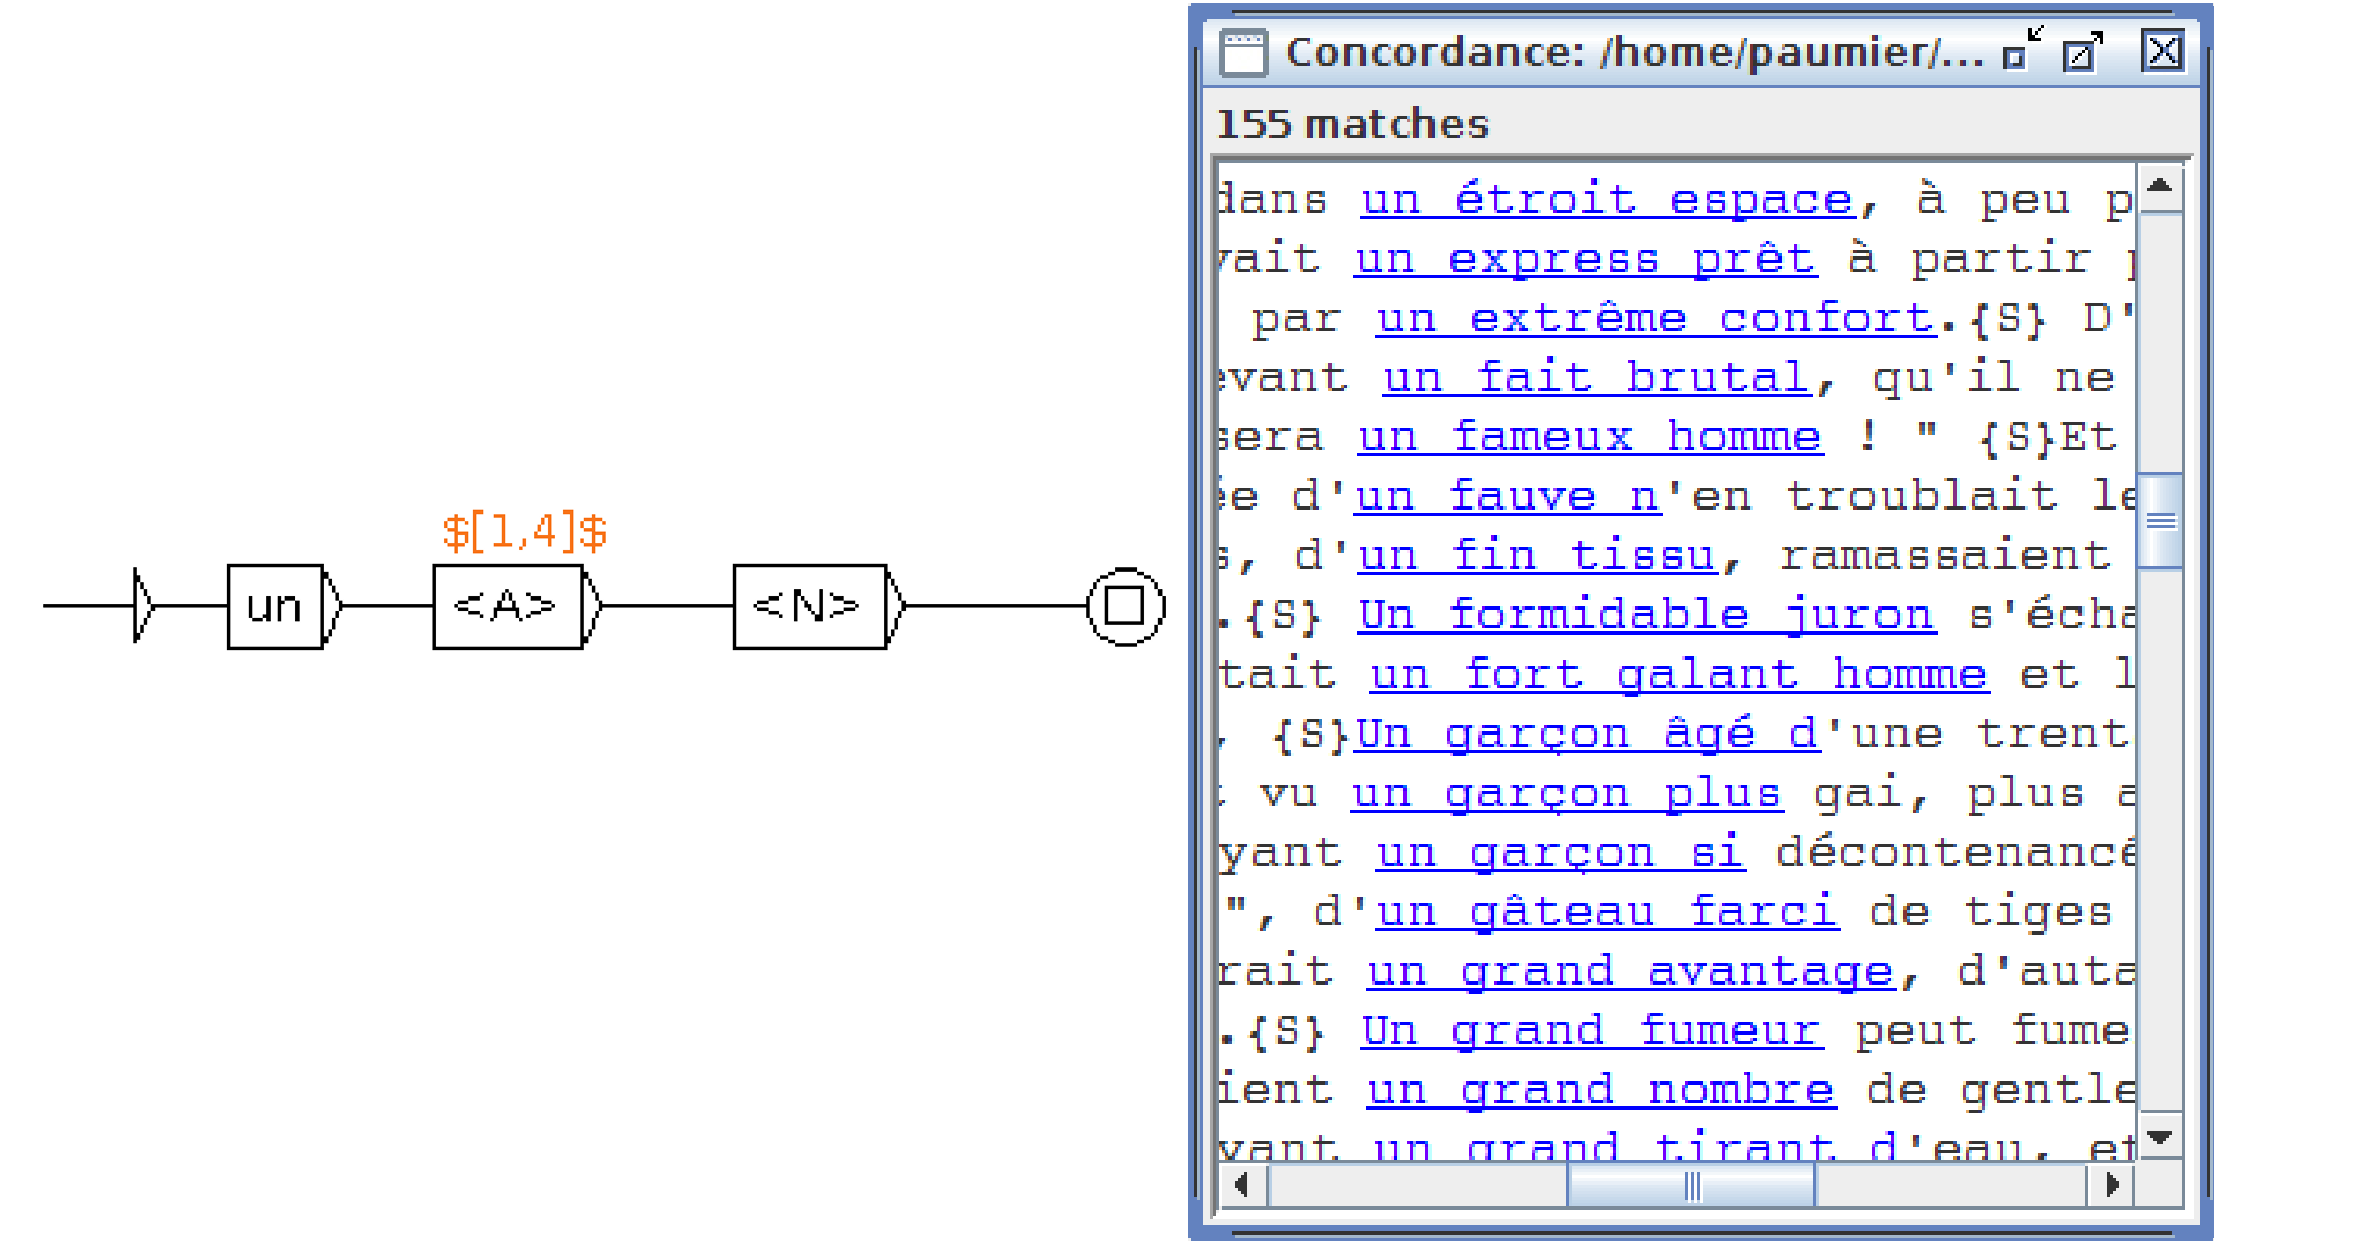
\includegraphics[width=13.5cm]{resources/img/fig6-10a.png}
\caption{Use of an interval to match several consecutive tokens\label{intervals}}
\end{center}
\end{figure}

\subsection{Error detection}
\index{Error detection in graphs}\index{Graph!detection of
errors}\index{Errors in graphs}
In order to keep the programs from blocking or crashing, Unitex automatically
detects errors during graph compilation. The graph compiler checks that the
main graph does not recognize the empty word and searches for all possible
forms of void loops. When an error is encountered, an error message is
displayed in the compilation window. Figure~\ref{fig-error-message} shows
the message that appears if one tries to compile the graph \verb+Det+ of
Figure~\ref{fig-recursive-calls-loop}.

\begin{figure}[!h]
\begin{center}
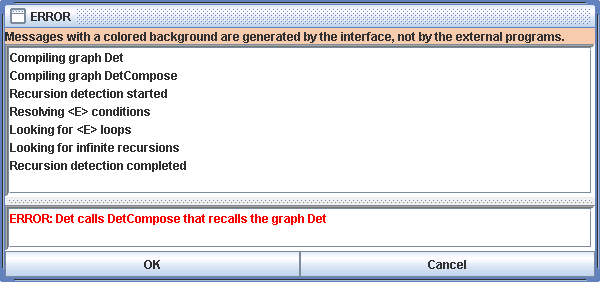
\includegraphics[width=15cm]{resources/img/fig6-11.png}
\caption{Error message when trying to compile
\texttt{Det}\label{fig-error-message}}
\end{center}
\end{figure}

\noindent When you start a pattern search with a \verb+.grf+
graph \index{File!\verb+.grf+}, if Unitex detects an error at the graph
compilation, the locate operation is automatically interrupted.


\section{Contexts}
\index{Contexts}\label{section-contexts}

Unitex graphs as we described them up to there are equivalent to algebraic
grammars. These are also known as context-free grammars, because if you want to
match a sequence $A$, the context of $A$ is irrelevant. Thus, you cannot use a
contex-free graph for matching occurences of \verb+president+ not followed by
\verb+of the republic+.

\bigskip
\noindent However, you can draw graphs with positive or negative contexts. In
that case, graphs are no more equivalent to algebraic grammars, but to context-sensitive
grammars that do not have the same theoretical properties.

\subsection{Right contexts}
\index{\verb+$[+}
\index{\verb+$]+}
To define a right context, you must bound a zone of the graph with boxes
containing \verb+$[+ and \verb+$]+, which indicate the start and the end of the
right context. These bounds appear in the graph as green square brackets. Both
bounds of a right context must be located in the same graph.

\bigskip
\begin{figure}[!h]
\begin{center}
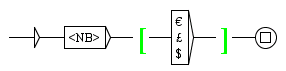
\includegraphics[width=7.4cm]{resources/img/fig6-12.png}
\caption{Using a right context\label{fig-context1}}
\end{center}
\end{figure}

\bigskip
\noindent Figure~\ref{fig-context1} shows a simple right context. The graph
matches numbers followed by a currency symbol, but this symbol will not appear in
matched sequences, \textit{i.e.} in the concordance.

\bigskip
\noindent Right contexts are interpreted as follows. During the application of a
grammar on a text, let us assume that a right context start is found. Let $pos$ be the
current position in the text at this time. Now, the \verb$Locate$ program tries to match
the expression described inside the right context. If it fails, then there will
be no match. If it matches the whole right context (that is to say if
\verb$Locate$ reaches the right context end), then the program will rewind at
the position \verb$pos$ and go on exploring the grammar after the right context
end.

\bigskip
\noindent You can also define negative right contexts,
using \verb+$![+ to indicate the right context start. Figure~\ref{fig-context2}
shows a graph that matches numbers that are not followed by \verb+th+. The difference
with positive right contexts is that when \verb$Locate$ tries to match the
expression described inside the context, reaching the context stop will be
considered as a failure, because it would have matched a forbidden sequence. At the opposite, if
the context stop cannot be reached, then \verb$Locate$ will rewind at the
position $pos$ and go on exploring the grammar after the context end.

\bigskip
\begin{figure}[!h]
\begin{center}
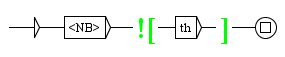
\includegraphics[width=7.3cm]{resources/img/fig6-13.png}
\caption{Using a negative right context\label{fig-context2}}
\end{center}
\end{figure}

\bigskip
\noindent Right contexts can appear anywhere in the graph, including the
beginning of the graph. Figure~\ref{fig-context3} shows a graph that matches an
adjective in the right context of something that is not a past participle. In other words, this
graph matches adjectives that are not ambiguous with past participles.

\bigskip
\begin{figure}[!h]
\begin{center}
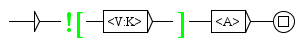
\includegraphics[width=7.5cm]{resources/img/fig6-14.png}
\caption{Matching an adjective that is not ambiguous with a past
participle\label{fig-context3}}
\end{center}
\end{figure}

\bigskip
\noindent This mechanism allows you to formulate complex patterns. For
instance, the graph of figure~\ref{fig-context4} matches a sequence of two 
simple nouns that is not ambiguous with a compound word. In fact, the 
pattern \verb?<CDIC><<^([^ ]+ [^ ]+)$>>? 
matches a compound word with exactly one space, and the pattern 
\verb?<N><<^([^ ]+)$>>? matches a noun without space, that is to say a simple 
noun. Thus, in the sentence \textit{Black cats should like the town hall}, 
this graph will match \textit{Black cats}, but not \textit{town hall}, which is
a compound word.

\bigskip
\begin{figure}[!h]
\begin{center}
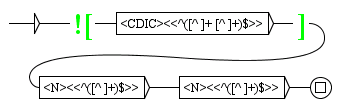
\includegraphics[width=8.9cm]{resources/img/fig6-15.png}
\caption{Advanced use of right contexts\label{fig-context4}}
\end{center}
\end{figure}

\bigskip
\noindent You can use nested contexts. For instance, the graph shown in
figure~\ref{fig-context5} matches a number that is not followed by a dot, except
for a dot followed by a number. Thus, in the sequence \textit{5.0+7.=12}, this graph
will match \textit{5}, \textit{0} and \textit{12}.

\bigskip
\begin{figure}[!h]
\begin{center}
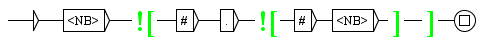
\includegraphics[width=12cm]{resources/img/fig6-16.png}
\caption{Nested contexts\label{fig-context5}}
\end{center}
\end{figure}

\bigskip
\noindent If a right context contains boxes with transducer outputs, the
outputs are ignored. However, it is possible to use a variable that was defined inside a
right context (cf. figure~\ref{fig-context6}). If you apply this graph in MERGE
mode to the text \textit{the cat is white}, you will obtain:

\bigskip
\texttt{the \textcolor{blue}{<pet name="cat" color="white"/>} is white}

\bigskip

\begin{figure}[!h]
\begin{center}
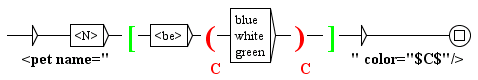
\includegraphics[width=12.2cm]{resources/img/fig6-17.png}
\caption{Variable defined inside a right context\label{fig-context6}}
\end{center}
\end{figure}

\subsection{Left contexts}
\index{\verb+$*+}
It is also possible to look for an expression $X$ only if it
occurs after an expression $Y$. Of course, it was already possible to do that with a grammar
like the one shown on Figure \ref{fig-left-context1}. However, with such a
grammar, the context part on the left will be included in the match, as shown on Figure
\ref{fig-left-context2}.

\begin{figure}[!ht]
\begin{center}
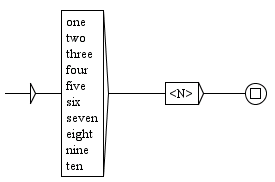
\includegraphics[width=7cm]{resources/img/fig6-17a.png}
\caption{Matching a noun that occurs after a numeral
determiner\label{fig-left-context1}}
\end{center}
\end{figure}

\begin{figure}[!ht]
\begin{center}
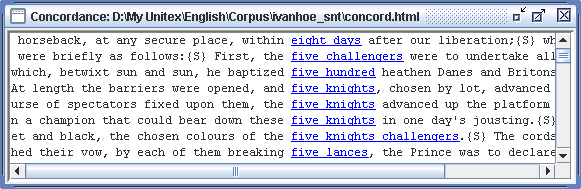
\includegraphics[width=14cm]{resources/img/fig6-17b.png}
\caption{Results of the application of the grammar shown on Figure
\ref{fig-left-context1}\label{fig-left-context2}}
\end{center}
\end{figure}

\bigskip
\noindent To avoid that, you can use the special symbol \verb+$*+ to indicate
the end of the left context of the expression you want to match. This symbol
will be represented by a green star in the graph, as shown on Figure
\ref{fig-left-context3}. The effect of such a context is to use this part of the
grammar for computing matches, but to ignore it in the results, as shown on
Figure \ref{fig-left-context4}.

\begin{figure}[!ht]
\begin{center}
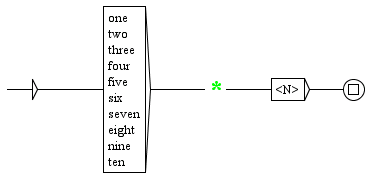
\includegraphics[width=9cm]{resources/img/fig6-17c.png}
\caption{Matching a noun after a left context\label{fig-left-context3}}
\end{center}
\end{figure}

\begin{figure}[!ht]
\begin{center}
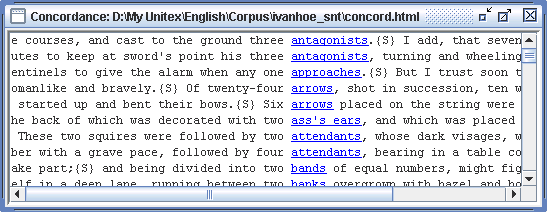
\includegraphics[width=14cm]{resources/img/fig6-17d.png}
\caption{Results of the application of the grammar shown on Figure
\ref{fig-left-context3}\label{fig-left-context4}}
\end{center}
\end{figure}

\clearpage
\noindent All the outputs produced in the left context are ignored, as you can
see in the concordance of Figure \ref{fig-left-context6}, showing the results
obtained with the grammar of Figure \ref{fig-left-context5}.

\begin{figure}[!ht]
\begin{center}
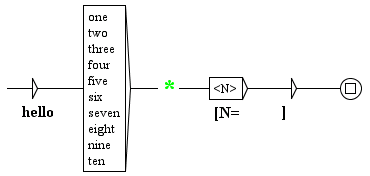
\includegraphics[width=9cm]{resources/img/fig6-17e.png}
\caption{Ignored output in a left context\label{fig-left-context5}}
\end{center}
\end{figure}

\begin{figure}[!ht]
\begin{center}
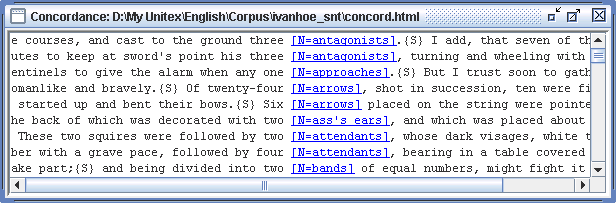
\includegraphics[width=15cm]{resources/img/fig6-17f.png}
\caption{Results of the application of the grammar shown on Figure
\ref{fig-left-context5}\label{fig-left-context6}}
\end{center}
\end{figure}

\bigskip
\noindent However, you can catch things with variables (see section
\ref{section-variables}) and use them outside the left context, as shown on the
grammar of Figure \ref{fig-left-context7} which produces the concordance of Figure \ref{fig-left-context8}.

\begin{figure}[!ht]
\begin{center}
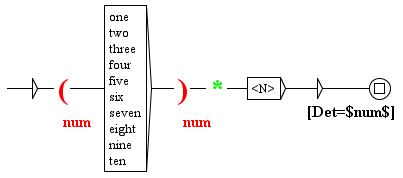
\includegraphics[width=10cm]{resources/img/fig6-17g.png}
\caption{Using a variable in a left context\label{fig-left-context7}}
\end{center}
\end{figure}

\begin{figure}[!ht]
\begin{center}
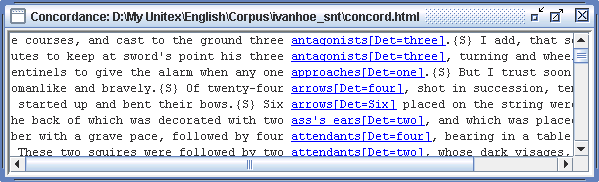
\includegraphics[width=15cm]{resources/img/fig6-17h.png}
\caption{Results of the application of the grammar shown on Figure
\ref{fig-left-context7}\label{fig-left-context8}}
\end{center}
\end{figure}

\bigskip
\noindent A graph with left contexts may be invoked in a grammar, but this requires caution.
When the left context part is excluded from the match, any sequences that had been matched before by 
any of the calling graphs are excluded from the match too, because the eventual matched sequence must be contiguous.
Any outputs in excluded sequences are ignored too.

\bigskip
\noindent Thus, with left and right contexts, you can make a distinction between
patterns used to match spots in texts, and the delimitation of the sequences to be extracted into your
results. For instance, the grammar shown on Figure \ref{fig-left-context9} looks
for expressions like \verb$the animal's$, but only extracts nouns, as you can
see on Figure \ref{fig-left-context10}.

\begin{figure}[!ht]
\begin{center}
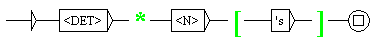
\includegraphics[width=10cm]{resources/img/fig6-17i.png}
\caption{A grammar with both left and right contexts\label{fig-left-context9}}
\end{center}
\end{figure}

\begin{figure}[!ht]
\begin{center}
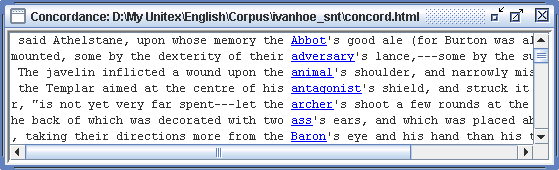
\includegraphics[width=15cm]{resources/img/fig6-17j.png}
\caption{Results of the application of the grammar shown on Figure
\ref{fig-left-context9}\label{fig-left-context10}}
\end{center}
\end{figure}

\clearpage

\section{The morphological mode}
\label{section-morphological-mode}
\index{Morphological mode}
\subsection{Why ?}
As Unitex works on a tokenized version of the text, it is not possible to
perform queries that need to enter inside tokens, except with morphological
filters (see section \ref{section-filters}), as shown on Figure
\ref{fig-morpho1}.

\begin{figure}[!ht]
\begin{center}
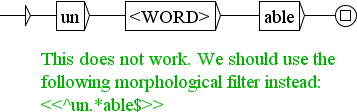
\includegraphics[width=8cm]{resources/img/fig6-17k.png}
\caption{Matching morphological elements\label{fig-morpho1}}
\end{center}
\end{figure}

\bigskip
\noindent However, even morphological filters cannot allow any query, since they
cannot refer to information stored in dictionaries. Thus, it is impossible to formulate this way a
query like ``\textit{a word made of the prefix} \verb$un$ \textit{followed by an
adjective suffixed with} \verb+able+''.

\bigskip
\noindent To overcome this difficulty, we introduced a morphological mode in
the \verb$Locate$ program. It consists of bounding a part of your grammar with
the special symbols \verb+$<+ and \verb+$>+.\index{\verb+$<+}\index{\verb+$>+}
Within this zone, sequences are matched letter by letter, as shown on Figure
\ref{fig-morpho2}.

\begin{figure}[!ht]
\begin{center}
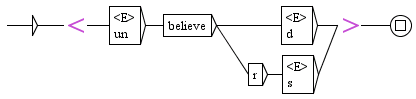
\includegraphics[width=11cm]{resources/img/fig6-17l.png}
\caption{Example of morphological zone in a grammar\label{fig-morpho2}}
\end{center}
\end{figure}

\subsection{The rules}
In this mode, the content of the graph is not interpreted as it is
in the normal way.
\begin{enumerate}
  \item There is no implicit space between boxes. So, if you
want to match a space, you have to make it explicit with \verb+" "+ (a space
between double quotes).

   \item You can still use subgraphs, but the end of the morphological zone
   must occur in the same graph as its beginning.

   \item You can use morphological filters on \verb+<DIC>+ and patterns
   referring to information stored in a dictionary, like \verb+<be>+, \verb+<N:ms>+, etc., provided
   that the dictionary has been previously declared as a morphological-mode dictionary
   (section~\ref{morph-mode-dic}).
   
   \item You can use morphological filters alone or on \verb+<TOKEN>+,
   but note that your filters will only apply to the current character. As a
   consequence, filters like \verb+<<[1-9][0-9]>>+ that are meant to match more than
   one character will never match anything. In fact, in morphological mode, 
   morphological filters should only be used to express negations like 
   \verb+<<[^aeiouy]>>+ (any character that is not a vowel). 
   
   \item Left and right contexts are forbidden.

   \item You can use outputs.
   
    \item \verb+<MOT>+ will match any letter, as defined in the alphabet
    file.\index{\verb+<MOT>+}

    \item \verb+<MIN>+ will match any lowercase letter, as defined in the
    alphabet file.\index{\verb+<MIN>+}

    \item \verb+<MAJ>+ will match any uppercase letter, as defined in the
    alphabet file.\index{\verb+<MAJ>+}

    \item \verb+<DIC>+ will match any word present in a morphological-mode
    dictionary\index{\verb+<DIC>+}, but the meta-symbols \verb+#+, \verb+<PRE>+, \verb+<NB>+, 
    \verb+<SDIC>+ and \verb+<CDIC>+ are forbidden.\index{\verb+#+} \index{\verb+<PRE>+}\index{\verb+<NB>+} \index{\verb+<TOKEN>+}  \index{\verb+<SDIC>+} \index{\verb+<CDIC>+}

    \item If you reach the end of the morphological zone and if you are not
    at the end of a token, the match will fail. For instance, if the text
    contains \verb+enabled+, you cannot match \verb+enable+ only.
\end{enumerate}


\subsection{Morphological-mode dictionaries}
\index{Morphological-mode dictionaries}
\label{morph-mode-dic}
In morphological mode, you can perform queries using dictionaries. For instance,  the grammar
of Figure~\ref{fig-morpho3} searches for every word made of the prefix \verb+un+ followed
by an adjective.

\begin{figure}[!ht]
\begin{center}
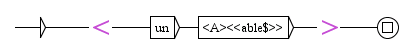
\includegraphics[width=11cm]{resources/img/fig6-17m.png}
\caption{Matching words made of 'un'+adjective ending with
'able'\label{fig-morpho3}}
\end{center}
\end{figure}

\begin{figure}[!ht]
\begin{center}
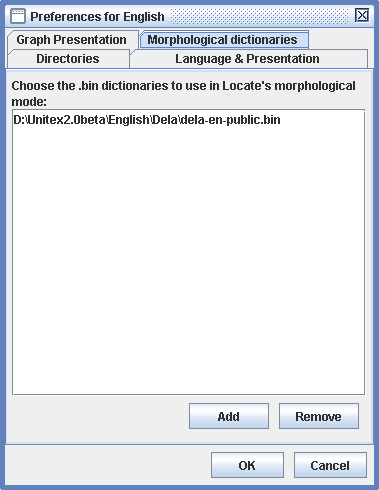
\includegraphics[width=11cm]{resources/img/fig6-17n.png}
\caption{Configuration of morphological-mode dictionaries\label{fig-morpho4}}
\end{center}
\end{figure}

\bigskip
\noindent To be able to match with this grammar the word 
\verb+unaware+, the system must know that \verb+aware+ is an adjective. But
\verb+aware+ may not be present in the text, so that we cannot rely on the text
dictionaries. This is the reason why we must define a list of dictionaries
to be looked up in the morphological mode. To do that, go in
``Info>Preferences>Morphological-mode dictionaries'', as shown on Figure
\ref{fig-morpho4}. You can select as many dictionaries as you want, but they
MUST be \verb+.bin+ ones. Once this is done, you can apply your grammar and get results.

\subsection{Dictionary-entry variables}
\index{Dictionary-entry variables}
\index{Variables!dictionary entry}
\label{dictionary-variables}
You can set variables to information stored in morphological-mode dictionaries.
The initialization of such a variable must be associated to a box that contains
a pattern referring to information stored in a morphological-mode dictionary,
except for the pattern \verb+<DIC>+. Set the output of the box with
\verb+$xxx$+ where \verb+xxx+ is a valid variable name (cf. section~\ref{section-using-variables}). That sets a
special variable named \verb+xxx+ to the dictionary entry that 
matches with your pattern. In the rest of the paths that contain the
box, you can get the inflected form, lemma and codes
of the entry with \verb+$xxx.INFLECTED$+, \verb+$xxx.LEMMA$+ and
\verb+$xxx.CODE$+, as shown on Figure \ref{fig-morpho5}. You can also use the
following patterns:
\begin{itemize}
  \item \verb+$xxx.CODE.GRAM$+: provides only the first grammatical code,
  supposed to be the POS category
  
  \item \verb+$xxx.CODE.SEM$+: provides all remaining grammatical codes, if any,
  separated with \verb$+$
  
  \item \verb+$xxx.CODE.FLEX$+: provides all inflectional codes, if
  any, separated with \verb$:$

  \item \verb+$xxx.CODE.ATTR=yyy$+: provides the value of an attribute-value pair contained in the semantic codes,
i.e. the value \verb+zzz+ of the \verb+yyy+ attribute if there is a code of the form \verb+yyy=zzz+.

\end{itemize}

\noindent Dictionary-entry variables can be used even after the end of the
morphological mode, as shown on Figure \ref{fig-morpho7}. They can also be
tested as explained in section \ref{section-variables}.
 
\begin{figure}[!ht]
\begin{center}
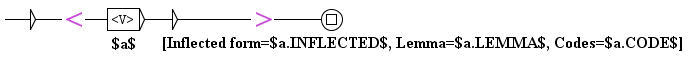
\includegraphics[width=16cm]{resources/img/fig6-17o.png}
\caption{Using a dictionary-entry variable\label{fig-morpho5}}
\end{center}
\end{figure}

\begin{figure}[!ht]
\begin{center}
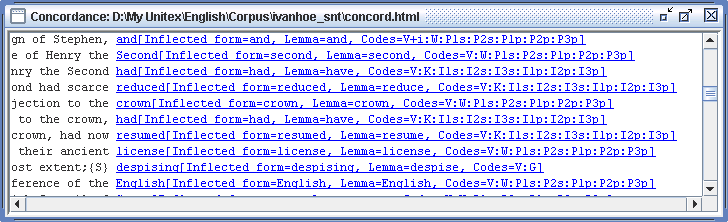
\includegraphics[width=15cm]{resources/img/fig6-17p.png}
\caption{Results of grammar of Figure \ref{fig-morpho5} applied in MERGE mode
\label{fig-morpho6}}
\end{center}
\end{figure}

\begin{figure}[!ht]
\begin{center}
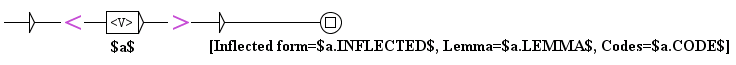
\includegraphics[width=15.5cm]{resources/img/fig6-17q.png}
\caption{Using a dictionary-entry variable in normal mode\label{fig-morpho7}}
\end{center}
\end{figure}


\bigskip
\noindent \textbf{Dictionary-entry variables in LocateTfst}

\noindent In grammars to be applied with \verb+LocateTfst+ (cf. section~\ref{section-locate-tfst}), you have an extra feature. 
If you are not in morphological mode, your grammar can extract information from a lexical tag contained in the text
automaton, and capture it into a dictionary-entry variable.
In your grammar, you have to set the output of a box with \verb+$:xxx$+, where
\verb+xxx+ is a valid variable name. In the rest of the paths that contain the
box, you can use \verb+xxx+ as a dictionary-entry variable, in the same way as
described above for the morphological mode: you can get from this variable the inflected form, lemma and codes
of the entry, its POS code, semantic codes,  inflectional codes and the value
 \verb+zzz+ of the \verb+yyy+ attribute if there is a code of the form \verb+yyy=zzz+.

\section{Exploring grammar paths}
\index{Exploring the paths of a grammar}

It is possible to generate the paths recognized by a grammar, if they are in
finite number, for example to check that it correctly generates the expected
forms. For that, open the main graph of your grammar, and ensure that the graph
window is the active window (the active window has a blue title bar, while the
inactive windows have a gray title bar). Now go to the "FSGraph" menu and then to
the "Tools" menu, and click on "Explore Graph paths". The Window of
figure~\ref{fig-explore-graph-paths} appears.


\begin{figure}[!h]
\begin{center}
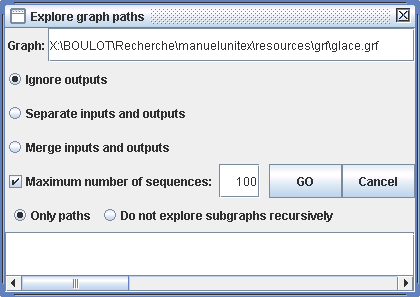
\includegraphics[width=10.4cm]{resources/img/fig6-18.png}
\caption{Exploring the paths of a grammar\label{fig-explore-graph-paths}}
\end{center}
\end{figure}

\bigskip
\noindent The upper box contains the name of the main graph of the grammar to be
explored. The following options are connected to the outputs of the grammar and
to subgraph calls:

\begin{itemize}
  \item "Ignore outputs": outputs are ignored;
  \item "Separate inputs and outputs": outputs are displayed after inputs
  (\verb$ a b c / A B C$);
  \item "Merge inputs and outputs": each output is emitted immediately after
  the input to which it corresponds  (\verb$a/A b/B c/C$).
  \item "Only paths": calls to subgraphs are explored recursively;
  \item "Do not explore subgraphs recursively": calls to subgraphs are printed
  but not explored recursively.
\end{itemize}

\noindent If the option "Maximum number of sequences" is activated, the
specified number will be the maximum number of generated paths. If the 
option is not selected, all
paths will be generated, if they are in finite number.

\bigskip
\noindent Here you see what is created for the graph shown on
Figure~\ref{fig-glace} with default settings (ignoring outputs, limit = 100
paths):

\bigskip
\noindent
\texttt{<NB> <boule> de glace \`a la pistache}

\noindent
\texttt{<NB> <boule> de glace \`a la fraise}

\noindent
\texttt{<NB> <boule> de glace \`a la vanille}

\noindent
\texttt{<NB> <boule> de glace vanille}

\noindent
\texttt{<NB> <boule> de glace fraise}

\noindent
\texttt{<NB> <boule> de glace pistache}

\noindent
\texttt{<NB> <boule> de pistache}

\noindent
\texttt{<NB> <boule> de fraise}

\noindent
\texttt{<NB> <boule> de vanille}

\noindent
\texttt{glace \`a la pistache}

\noindent
\texttt{glace \`a la fraise}

\noindent
\texttt{glace \`a la vanille}

\noindent
\texttt{glace vanille}

\noindent
\texttt{glace fraise}

\noindent
\texttt{glace pistache}

\begin{figure}[!h]
\begin{center}
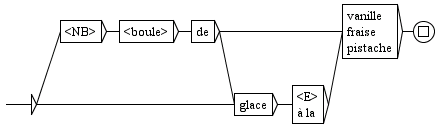
\includegraphics[width=10.9cm]{resources/img/fig6-19.png}
\caption{Sample graph \label{fig-glace}}
\end{center}
\end{figure}




\section{Graph collections}
\index{Collections of graphs}

It can happen that one wants to apply several grammars located in the same directory. For
that, it is possible to automatically build a grammar starting from a file tree
structure. Let us suppose for example that one has the following tree structure:

\begin{itemize}
  \item \textit{Dicos}:
  \begin{itemize}
    \item \textit{Banque}:
    \begin{itemize}
      \item \texttt{carte.grf}
    \end{itemize}
    \item \textit{Nourriture}:
    \begin{itemize}
      \item \texttt{eau.grf}
      \item \texttt{pain.grf}
    \end{itemize}
    \item \texttt{truc.grf}
  \end{itemize}
\end{itemize}

\noindent If one wants to gather all these grammars in only one, one can do it
with the "Build Graph Collection" command in the "FSGraph Tools" sub-menu. One configures
this operation by means of the window seen in
figure~\ref{fig-build-graph-collection}.

\begin{figure}[!h]
\begin{center}
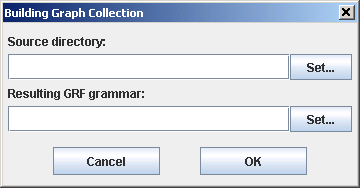
\includegraphics[width=9cm]{resources/img/fig6-20.png}
\caption{Building a graph collection\label{fig-build-graph-collection}}
\end{center}
\end{figure}

\noindent In the "Source Directory" field, select the root directory which you
want to explore (in our example, the directory \textit{Dicos}). In the field "Resulting
GRF grammar", enter the name of the produced grammar.

\bigskip
\noindent WARNING: Do not place the output grammar in the tree structure which
you want to explore, because in this case the program will try to read and to write
simultaneously in this file, which will cause a crash.

\bigskip
\noindent When you click on "OK", the program will copy the graphs to the directory of the
output grammar, and will create subgraphs corresponding to the various
sub-directories, as one can see in figure~\ref{fig-graph-collection}, which
shows the output graph generated for our example.

\bigskip
\noindent One can observe that one box contains the calls with subgraphs corresponding to
sub-directories (here directories \textit{Banque} and \textit{Nourriture}), and
that the other box calls  all the graphs which were in the directory (here the
graph \texttt{truc.grf}).

\begin{figure}[!h]
\begin{center}
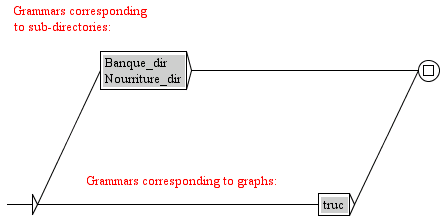
\includegraphics[width=11cm]{resources/img/fig6-21.png}
\caption{Main graph of a graph collection\label{fig-graph-collection}}
\end{center}
\end{figure}



\section{Rules for applying transducers}
\label{section-applying-transducers-rules}
\index{Transducer!rules for application}\index{Rules!for transducer application}
This section describes the rules for the application of transducers along with
the operations of preprocessing and the search for patterns. The following does
not apply to inflection graphs and normalization graphs for ambiguous forms.

\subsection{Insertion to the left of the matched pattern}
\index{MERGE}\index{REPLACE}
When a transducer is applied in REPLACE mode, the output replaces the sequences
that have been read in the text. When a box in a transducer has no
output, it is processed as if it had an \verb+<E>+ output. In MERGE mode, the
output is inserted to the left of the recognized sequences. 

\begin{figure}[!h]
\begin{center}
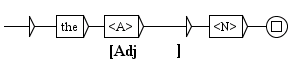
\includegraphics[width=7.2cm]{resources/img/fig6-22.png}
\caption{Example of a transducer\label{fig-transducer-example}}
\end{center}
\end{figure}

\bigskip
\noindent Look at the transducer in Figure~\ref{fig-transducer-example}.
If this transducer is applied to the novel \textit{Ivanhoe} by Sir Walter Scott
in MERGE mode, the following concordance is obtained.

\begin{figure}[!h]
\begin{center}
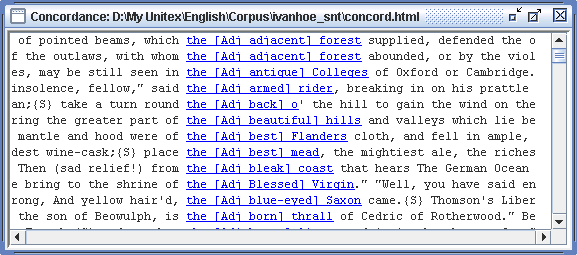
\includegraphics[width=14.4cm]{resources/img/fig6-23.png}
\caption{Concordance obtained in MERGE mode with the transducer of
figure~\ref{fig-transducer-example}}
\end{center}
\end{figure}

\subsection{Application while advancing through the text}
During the preprocessing operations, the text is modified as it is being read.
In order to avoid the risk of infinite loops, it is necessary that the
sequences that are produced by a transducer will not be re-analyzed by the same one.
Therefore, whenever a sequence is inserted into the text, the application of the
transducer is continued after that sequence. This rule
only applies to  preprocessing transducers, because during the
application of syntactic graphs, the transductions do not modify the processed
text but a concordance file which is distinct from the text.

\subsection{Priority of the leftmost match}
\label{section-priority-leftmost-match}
\index{Priority!of the leftmost match} \index{Overlapping occurrences}
During the application of a local grammar, overlapping occurrences
are all indexed. Note that we talk about real overlapping occurrences like
\verb+abc+ and \verb+bcd+, not nested occurrences like \verb+abc+ and
\verb+bc+. During the construction of the concordance all these overlapping 
occurrences are presented (cf. Figure~\ref{fig-overlappping-occurrences}).

\begin{figure}[!h]
\begin{center}
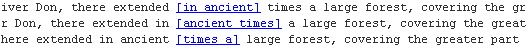
\includegraphics[width=13cm]{resources/img/fig6-24.png}
\caption{Overlapping occurrences in concordance\label{fig-overlappping-occurrences}}
\end{center}
\end{figure}

\noindent On the other hand, if you modify a text instead of constructing a
concordance, it is necessary to choose among these occurrences the one  that will be taken into account.
Unitex applies the following priority rule for that purpose: the leftmost
sequence is used.

\bigskip
\noindent If this rule is applied to the three occurrrences of the preceding
concordance, the occurrence \textcolor{blue}{\texttt{[in ancient]}} overlaps with
\textcolor{blue}{\texttt{[ancient times]}}. The first  is retained because this
is the leftmost occurrence and \textcolor{blue}{\texttt{[ancient times]}} is
eliminated. The following occurrence of \textcolor{blue}{\texttt{[times a]}} is
no longer in conflict with \textcolor{blue}{\texttt{[ancient times]}} and can
therefore appear in the result:
\begin{center}
\texttt{...Don, there extended \textcolor{blue}{[in ancient] [times a]} large forest...}
\end{center}

\noindent The rule of priority of the leftmost match is applied only when the
text is modified, be it during preprocessing or after the application of a syntactic
graph (cf. section~\ref{section-modifying-text}).

\subsection{Priority of the longest match}
\index{Priority!of the longest match}
During the application of a syntactic graph it is possible to choose if the
priority should be given to the shortest or the longest sequences or if all
sequences should be retained. During preprocessing, the priority is always given
to the longest sequences.


\subsection{Transducer outputs with variables}
\label{section-variables}
\index{Variables!in graphs}\index{Transducer output!with variables}
As we have seen in section~\ref{section-using-variables}, it is
possible to use input variables to store some text that has been analyzed by a
grammar. Such variables can be used in preprocessing graphs and in syntactic
graphs.

\bigskip
\noindent You have to give names to the variables you use. These names can
contain non-accentuated lower-case and upper-case letters between \verb+A+ and \verb+Z+,
digits and the character \verb+_+ (underscore).\index{Underscore}

\bigskip
\noindent In order to delimit the zone to be stored in an input
variable, you have to create two boxes that contain the name of the variable 
enclosed in the characters \verb-$- and \verb-(- (\verb-$- and \verb-)- for the end of a
variable). In order to use a variable in a transducer output, its name must be
surrounded by the character \verb-$- (cf. Figure~\ref{fig-variable-definition}).

\bigskip
\noindent Variables are global. This means that you can define a variable in a graph and
reference it in another as is illustrated in the graphs of
Figure~\ref{fig-variable-definition}.

\begin{figure}[!p]
\begin{center}
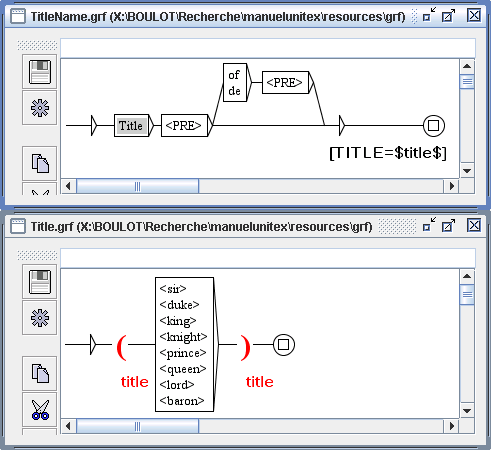
\includegraphics[width=12cm]{resources/img/fig6-25.png}
\caption{Definition of an input variable in a subgraph\label{fig-variable-definition}}
\end{center}
\end{figure}

\bigskip
\noindent If the graph \verb+TitleName+ is applied in MERGE mode to the text
\textit{Ivanhoe}, the concordance in Figure~\ref{fig6-14} is obtained.

\begin{figure}[!p]
\begin{center}
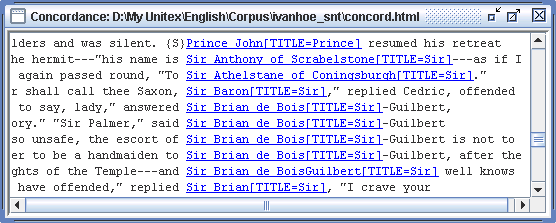
\includegraphics[width=13.5cm]{resources/img/fig6-26.png}
\caption{Concordance obtained by application of graph \texttt{TitleName}\label{fig6-14}}
\end{center}
\end{figure}

\index{Moving phrases}
\bigskip
\noindent Outputs with variables can be used to move phrases. In
fact, the application of a transducer in REPLACE mode inserts only the produced sequences
into the text. In order to swap two phrases, you just have to
store them into variables and produce an output with these variables in the
desired order. Thus, the application of the transducer in
Figure~\ref{fig-swapping-words} in REPLACE mode to the text \textit{Ivanhoe}
results in the concordance of
Figure~\ref{fig-no-space-problem}.

\begin{figure}[!ht]
\begin{center}
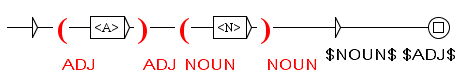
\includegraphics[width=11.3cm]{resources/img/fig6-27.png}
\caption{Swapping words using two input variables\label{fig-swapping-words}}
\end{center}
\end{figure}

\begin{figure}[!ht]
\begin{center}
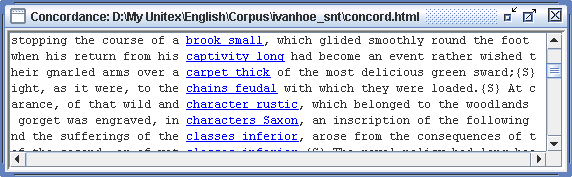
\includegraphics[width=13.4cm]{resources/img/fig6-28.png}
\caption{Result of the application of the transducer in 
figure~\ref{fig-swapping-words}\label{fig-no-space-problem}}
\end{center}
\end{figure}

\bigskip
\noindent If the beginning or the end of variable does not conform to the syntax above (end of a variable before
its beginning, or absence of the beginning or end of a variable), by default, it
will be ignored during the emission of outputs. See section
\ref{section-advanced-search-options} for other variable error policies.

\bigskip
\noindent There is no limit to the number of possible variables.

\bigskip
\noindent Input variables can be nested and even overlap as is shown in
figure~\ref{fig-overlapping-variables}.

\begin{figure}[!ht]
\begin{center}
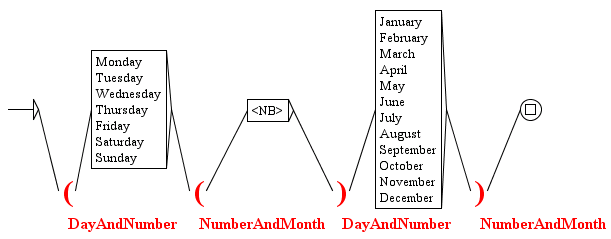
\includegraphics[width=15cm]{resources/img/fig6-29.png}
\caption{Overlapping input variables\label{fig-overlapping-variables}}
\end{center}
\end{figure}

\clearpage




\section{Output variables}
\label{section-output-variables}
\index{Output variables}
\index{Variables!output}
Input variables declared with \verb+$xxx(+ and \verb+$xxx)+ capture portions of the input text. It
is also possible to capture portions of the outputs produced by your grammar. This is done with output variables.
Such variables are declared with \verb+$|xxx(+ and \verb+$|xxx)+. Those tags appear in blue as shown 
on Figure \ref{fig-output-variables}. Note that when an output variable is being initialized, the output sequences
of the transducer
are not emitted into the output for the current occurrence; they are just stored into the pending output variable(s).
Note that outputs are processed first, so that if an output string contains something like \verb+$A.LEMMA$+,
the output variable will not contain this raw string but rather the lemma associated to variable \verb+A+.
Moreover, output variables only capture explicit outputs produced by your grammar. Thus, even if you work
in MERGE mode, output variables never capture the input text. 

\noindent For instance, this example grammar applied to \textit{Ivanhoe} will produce in MERGE mode the concordance 
shown on Figure \ref{fig-output-variables-concord}. Thus you can see that the outputs \verb+ADJ+ and 
\verb+NOUN+ have not been inserted to the left of the input text, as one may have expected.

\begin{figure}[!ht]
\begin{center}
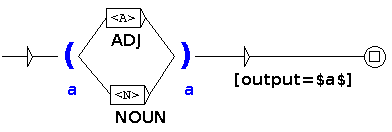
\includegraphics[width=8cm]{resources/img/fig6-17r.png}
\caption{Output variables\label{fig-output-variables}}
\end{center}
\end{figure}

\begin{figure}[!ht]
\begin{center}
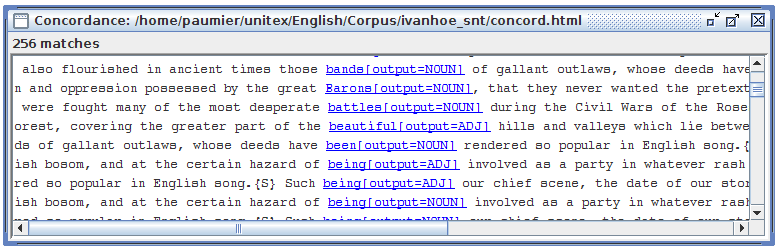
\includegraphics[width=15cm]{resources/img/fig6-17s.png}
\caption{Concordance obtained with grammar of Figure \ref{fig-output-variables}\label{fig-output-variables-concord}}
\end{center}
\end{figure}


\section{Operations on variables}
\label{section-ops-on-variables}
\subsection{Testing variables}
\index{Testing variables}\index{Variables!test}

\noindent It is possible to test whether a variable has been defined or not, in
order to block the current matching operation if the condition is not verified.
This is done by inserting the sequence \verb+$xxx.SET$+ in the output of a
graph box. Then, if a variable named \verb+xxx+ has been defined, this sequence
will be ignored in the output and the matching process will go on; otherwise, matching
will be stopped and the program will backtrack. This operates on
input variables as well as on output variables and dictionary-entry variables defined in
morphological mode. You can check out if a variable has not been defined in the
same way using \verb+$xxx.UNSET$+. Figure \ref{fig-testing-a-variable} shows
a graph that use a such a variable test. Figure
\ref{fig-testing-a-variable-results} shows results obtained with this graph in
MERGE mode.

\begin{figure}[!ht]
\begin{center}
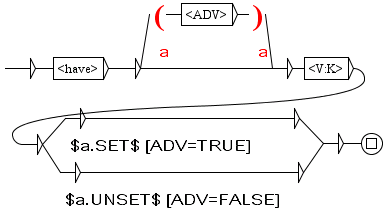
\includegraphics[width=9cm]{resources/img/fig6-29b.png}
\caption{Testing a variable\label{fig-testing-a-variable}}
\end{center}
\end{figure}

\begin{figure}[!ht]
\begin{center}
\includegraphics[width=10cm]{resources/img/fig6-29c.png}
\caption{Results of a variable test\label{fig-testing-a-variable-results}}
\end{center}
\end{figure}


\subsection{Comparing variables}
\index{Comparing variables}
\index{Variables!comparison}
Another kind of test you can perform consists of variable comparison.
You can compare a variable of any kind (whether an input variable, an output variable or a dictionary-entry variable)
against a constant string or another variable. To do that, you have to use the following syntax:

\bigskip
\noindent \verb+$abc.EQUAL=xyz$+

\bigskip
\noindent This acts like a switch that will block the grammar exploration if the value of variable \verb+abc+
is different from the value of variable \verb+xyz+. Note that for dictionary-entry variables,
what is used in the test is the inflected form
as found in the dictionary (beware of case variations!). If you want to compare variable
\verb+abc+ against the constant string \verb+JKL+, use the following test:

\bigskip
\noindent \verb+$abc.EQUAL=#JKL$+

\bigskip
\noindent You can also test if contents differ with \verb+UNEQUAL+.

\bigskip
\noindent If you want to compare variables so that case variations are ignored, you can use the following tests:

\bigskip
\noindent \verb+$abc.EQUALcC=xyz$+ \\
or \\
\verb+$abc.UNEQUALcC=xyz$+

\section{Applying graphs to texts}
\label{section-applying-graphs-to-text}
This section only applies to syntactic graphs.
\subsection{Configuration of the search}
In order to apply a graph to a text, you open the text, then click on "Locate
Pattern..." in the "Text" menu, or press <Ctrl+L>. You can then configure your
search in the window shown in figure~\ref{fig-regexp-frame}.

\bigskip
\index{Search for patterns}
\noindent In the "Locate pattern in the form of" field, choose "Graph" and
select your graph by clicking on the "Set" button. You can choose a graph in \verb+.grf+
format (Unicode Graphs) or a compiled graph in \verb+.fst2+ format (Unicode
Compiled Graphs). If your graph is a \verb+.grf+ one, Unitex will compile it
automatically before starting the search. If you click on "Activate debug mode", the 
concordance will be displayed in a window in which you will also find the automaton and, 
for each match, the list of states of the path that matches it. This window is described
with more details in section~\ref{section-debug-mode}.

\bigskip
\noindent The "Index" field allows to select the recognition mode.

\bigskip
\index{Shortest matches}\index{Longest matches}\index{All matches}
\begin{itemize}
  \item "Shortest matches" : give precedence to the shortest matches;
  \item "Longest matches" : give precedence to the longest sequences. This is the
  default mode;
  \item "All matches" : give out all recognized sequences.
\end{itemize}

\bigskip
\noindent 
The "Search limitation" field allows you to limit the search to a certain number of
occurrences. By default, the search is limited to the 200 first
occurrences.\index{Occurrences!number of}

\bigskip
\begin{figure}[!h]
\begin{center}
\includegraphics[width=9cm]{resources/img/fig6-30.png}
\caption{Locate pattern Window\label{fig-regexp-frame}}
\end{center}
\end{figure}

\index{MERGE}\index{REPLACE}
\noindent The "Grammar outputs" field concerns transducers. The "Merge with
input text" mode allows you to insert the output sequences in input sequences.
The "Replace recognized sequences" mode allows you to replace the 
recognized sequences with the produced sequences. The third mode ignores all
outputs. This latter mode is used by default.

\bigskip
\noindent
In the "Search algorithm" frame, you can specify wether you want to perform the locate 
operation on the text using the Locate program or on the text automaton with LocateTfst.
By default, search is done with the Locate program, as Unitex always did until now. If you
want to use LocateTfst, please read dedicated section~\ref{section-locate-tfst}.
\bigskip
\noindent
After you have selected the parameters, click on "SEARCH" to start the search.

\clearpage
\subsection{Advanced search options}
\index{Advanced search options}
\label{section-advanced-search-options}
If you select the "Advanced options" tab, you will see the frame shown on
Figure \ref{fig6-advanced-options1}.

\bigskip
\begin{figure}[!h]
\begin{center}
\includegraphics[width=9cm]{resources/img/fig6-advanced-options1.png}
\caption{Advanced search options\label{fig6-advanced-options1}}
\end{center}
\end{figure}

\index{Ambiguous outputs}
\noindent The "Ambiguous output policy" option can be illustrated with the
graph shown on Figure \ref{fig6-advanced-options2}. When a determiner is
followed by a word that can be either adjective or noun, it can produce two
distinct outputs for the same text input sequence.

\bigskip
\begin{figure}[!h]
\begin{center}
\includegraphics[width=9cm]{resources/img/fig6-advanced-options2.png}
\caption{A graph with ambiguous outputs\label{fig6-advanced-options2}}
\end{center}
\end{figure}

\noindent If we apply this graph on \textit{Ivanhoe} with the "Allow ambiguous
outputs" option (the default one), we will obtain the text order
concordance shown of Figure \ref{fig6-advanced-options3}. As you can see, two
outputs have been produced for the input sequence \textit{the noble}.

\bigskip
\begin{figure}[!h]
\begin{center}
\includegraphics[width=8.8cm]{resources/img/fig6-advanced-options3.png}
\caption{Ambiguous outputs for \textit{the noble}\label{fig6-advanced-options3}}
\end{center}
\end{figure}


\noindent At the opposite, with the "Forbid ambiguous
outputs" option, we will obtain the text order
concordance shown of Figure \ref{fig6-advanced-options4}, with only one
arbitrarily chosen output for the input sequence \textit{the noble}.

\bigskip
\begin{figure}[!h]
\begin{center}
\includegraphics[width=9cm]{resources/img/fig6-advanced-options4.png}
\caption{Single output for \textit{the noble}\label{fig6-advanced-options4}}
\end{center}
\end{figure}


\index{Variable error policy}
\bigskip
\noindent The "Variable error policy" option allows you to specify what
\verb+Locate+/\verb+LocateTfst+ is supposed to do when an output is found that
contains a reference to a variable that has not been correctly defined. Note
that this parameter has no effect if outputs are to be ignored. 
For instance, let us consider the graph shown on Figure
\ref{fig6-advanced-options5}. 

\bigskip
\begin{figure}[!h]
\begin{center}
\includegraphics[width=9cm]{resources/img/fig6-advanced-options5.png}
\caption{A variable \textit{A} that may be
undefined\label{fig6-advanced-options5}}
\end{center}
\end{figure}

\noindent With the "Ignore variable errors" option, \textit{A} will just be
ignored, as if it had an empty content, as shown on Figure
\ref{fig6-advanced-options6}. 

\bigskip
\begin{figure}[!h]
\begin{center}
\includegraphics[width=12cm]{resources/img/fig6-advanced-options6.png}
\caption{
 variable \textit{A} that may be
undefined\label{fig6-advanced-options6}}
\end{center}
\end{figure}


\noindent With the "Exit on variable error" option, \verb+Locate+/\verb+LocateTfst+
will exit with an error message, as shown on Figure
\ref{fig6-advanced-options7}.

\bigskip
\begin{figure}[!h]
\begin{center}
\includegraphics[width=9cm]{resources/img/fig6-advanced-options7.png}
\caption{Exiting on variable error\label{fig6-advanced-options7}}
\end{center}
\end{figure}

\noindent With the "Backtrack on variable error" option,
\verb+Locate+/\verb+LocateTfst+ will stop exploring the current path in the
grammar. Thus, variables play the role of switches that cut paths
when variables are undefined. For instance, the application of grammar
\ref{fig6-advanced-options5} will only produce matches containing an adjective, as shown on Figure 
\ref{fig6-advanced-options8}. 

\bigskip
\begin{figure}[!h]
\begin{center}
\includegraphics[width=13cm]{resources/img/fig6-advanced-options8.png}
\caption{Backtracking on variable error\label{fig6-advanced-options8}}
\end{center}
\end{figure}



\subsection{Concordance}
\index{Concordance}
The result of a search is an index file that contains the positions of all
encountered occurrences.
The window of Figure~\ref{fig-configuration-display-occurrences} lets you
choose whether to construct a concordance or modify the text.

\bigskip
\index{Contexts!concordance}\index{Sorting!of concordances}
\noindent In order to display a concordance, you have to click on the "Build
concordance" button. You can parameterize the size of left and right contexts in characters.
You can also choose the sorting mode that will be applied to the lines of the
concordance in the "Sort According to" menu. For further details on the
parameters of concordance construction, refer to
section~\ref{section-display-occurrences}.
%\bigskip
\begin{figure}[h]
\begin{center}
\includegraphics[width=10cm]{resources/img/fig6-31.png}
\caption{Configuration for displaying the encountered occurrences
\label{fig-configuration-display-occurrences}}
\end{center}
\end{figure}
\noindent The concordance is produced in the form of an HTML file.
\index{File!HTML} You can parameterize Unitex  so that concordance files 
can be read using a web browser
(cf. section~\ref{section-display-occurrences}).\index{Web browser}

\bigskip
\noindent If you display concordances with the window provided by Unitex,
you can access a recognized sequence in the text by clicking on the occurrence. If
the text window is not iconified and the text is not too long to be displayed,
you see the selected sequence appear (cf.
Figure~\ref{fig-back-to-text}).

%\bigskip
\begin{figure}[h]
\begin{center}
\includegraphics[width=13.5cm]{resources/img/fig6-32.png}
\caption{Selection of an occurrence in the text\label{fig-back-to-text}}
\end{center}
\end{figure}

\noindent Furthermore, if the text automaton has been constructed, and if the
corresponding window is not iconified, clicking on an occurrence selects the automaton of the
sentence that contains this occurrence.

\subsection{Modification of the text}
\label{section-modifying-text}
\index{Text!modification}\index{Modification of the text}
You can choose to modify the text instead of constructing a concordance. In order
to do that, type a file name in the "Modify text" field in the window of
Figure~\ref{fig-configuration-display-occurrences}. This file has to have the
extension \verb+.txt+.
\index{File!\verb+.txt+}

\bigskip
\noindent If you want to modify the current text, you have to choose the
corresponding \verb+.txt+ file. If you choose another file name, the current text will not be
affected. Click on the  "GO" button to start the modification of the text. The
precedence rules that are applied during these operations are described in
section~\ref{section-applying-transducers-rules}.

\bigskip
\noindent After this operation, the resulting file is a copy of the text
in which transducer outputs have been taken into account. Normalization
operations and splitting into lexical units are automatically applied to
this text file. The existing text dictionaries are not modified. Thus, if you
have chosen to modify the current text, the modifications will be effective
immediately. You can then start new searches on the text.

\bigskip
\noindent WARNING: if you have chosen to apply your graph ignoring the
transducer outputs, all occurrences will be erased from the text.




\subsection{Extracting occurrences}
\index{Extracting occurrences}\index{Occurrences!extraction}
To extract from a text all sentences containing matches, set the name of your
output text file using the "Set File" button in the "Extract units" frame (Figure
\ref{fig-configuration-display-occurrences}). Then, click on "Extract matching
units". At the opposite, if you click on "Extract unmatching units", all
sentences that do not contain any match will be extracted.


\subsection{Comparing concordances}
\label{section-comparing-concordances}
\index{Comparing concordances}\index{Concordance!comparison}\index{External programs!\verb+ConcorDiff+}
\index{\verb+ConcorDiff+}
With the "Show differences with previous concordance" option, you can compare the current
concordance with the previous one. The  \verb+ConcorDiff+ program builds both concordances
according to text order and compares them line by line. The result is an HTML page that
presents alternatively lines from both concordances, leaving an empty line when a match
 appears in only one concordance. 
Lines are greyed for the previous concordance and left with a white background for the current one.
In each line, only matched tokens are coloured. You can click on each match to open the text at its position. Figure~\ref{fig-concordiff} gives an example.

\begin{figure}[h]
\begin{center}
\includegraphics[width=10cm]{resources/img/fig6-33.png}
\caption{Example of a concordance comparison\label{fig-concordiff}}
\end{center}
\end{figure}

\bigskip
\noindent Blue indicates that an occurrence is common to the two concordances. Red indicates that a match is common but
with a different range, i.e. the two matches only overlap partially. Green indicates an
occurrence that appears in only one concordance.

\bigskip
\noindent If you have no previous concordance the button is deactivated.

%\clearpage
\subsection{Debug mode}
\label{section-debug-mode}
When  you apply a graph to a text with the Locate menu 
in the window shown in figure~\ref{fig-regexp-frame}, 
%you can display a concordance in which the located sequences 
if you activate the debug mode in the "Locate pattern in the forme of" field,
the concordance will be displayed in a special window such as in figure~\ref{fig-debug-mode}, divided into three parts :

\medskip 
\indent In the top right part of the window is the concordance. It is identical to the classical concordance in which the sequences matched by the graph appear in blue.

\medskip
\indent In the bottom right you will find the graph used for the locate.

\medskip
\indent In the left side of the window is a table of 3 columns : "Tag", "output" and "matched".
Each token of the matched sequence appear in the "matched" column, the Tag column contains what is in the box of the automaton that matched it, and if this box has any output, it will appear in the "output" column.

\bigskip
\noindent For each matched sequence in the concordance, if you click on its line in the concordance, the table on the left will be actualized and clicking on a row of the table will colour the corresponding box in the graph.
\bigskip
\noindent This will help you to see, for each occurence of a matched sequence in the text, which path in the automaton recognized it. A red number above each box indicates the number of sequences in the text in which that box matched a token. 


%\bigskip
\begin{figure}[h]
\begin{center}
\includegraphics[height=9cm]{resources/img/fig6-34.png}
\caption{The Concordance window in debug mode\label{fig-debug-mode}}
\end{center}
\end{figure}
